\section{Equilibrium with an upper bound on AI efficiency}
\label{sec:rewrite-regimes}

In this section, I characterize the long-run equilibrium behavior for various parameter configurations. The key finding is that long-run output-per-worker growth can exceed the rate of labor-augmenting technological change when the elasticity of substitution between AI production services and labor exceeds one and the upper bound on AI efficiency is sufficiently high.

To identify this threshold, I calculate the net return on capital implied by the production and pricing conditions as AI efficiency approaches its upper bound and labor's income share tends to zero. I compare this return with $\rho+\gamma$, the interest rate that sustains consumption-per-person growth at the exogenous rate $\gamma$. When the former exceeds the latter and AI and labor are substitutes, the model supports equilibrium paths along which capital and AI production services grow faster than effective labor, even though AI efficiency converges to a finite limit.
%The parameter restrictions used in all three propositions are
%\begin{equation}
% \begin{gathered}
% 0<\alpha<1,\quad 0<\eta<1,\quad \delta\geq0,\quad \chi>0,\\
% \omega_L,\omega_X>0,\quad \omega_L+\omega_X=1,\quad
% n\geq0,\quad \gamma>0,\quad \rho>n.
% \end{gathered}
% \label{eq:rewrite-finite-existence-parameters}
%\end{equation}
%These are the primitive restrictions in Section~\ref{sec:rewrite-model}.
%In particular, the local results with a finite upper bound do not require Assumptions~\ref{ass:rewrite-research-curvature} or \ref{ass:rewrite-research-concavity}. Sufficiently near the upper bound, its diminishing scope for improvement permits global verification of the developer's policy even when $\eta>1/2$.

%The inequality $n+\gamma>0$ already follows from \eqref{eq:rewrite-population} and \eqref{eq:rewrite-labor-productivity}, so it is not a separate assumption. It makes effective labor grow and gives the remaining AI-efficiency gap a positive asymptotic rate of closure in the constructions below. The case $n+\gamma=0$ is not covered by these proofs.

%Each proposition below states the restrictions on $\sigma$, the upper bound, and the initial stocks that are specific to its construction. The results do not concern the uncapped economy. They are local in initial stocks, not in time: each constructs a trajectory defined for every $t\geq0$, including both transversality conditions and agent optimality. The initial stocks need not lie on a balanced-growth path. The neighborhoods are in normalized coordinates and require initial AI efficiency sufficiently close to its upper bound. Local uniqueness below means uniqueness among solutions that remain near the indicated normalized long-run limit and converge to it; it does not exclude other equilibria outside that neighborhood.

\subsection{The return to capital and the efficiency threshold}
\label{subsec:rewrite-return-threshold}

An upper bound restricts AI efficiency, but not the compute used to supply AI production services. To identify the return when labor's income share vanishes, fix $B>0$ and consider $s_X\to1$. Since $wL/Y=(1-\alpha)(1-s_X)$, this is the zero-labor-share limit.

Combine the final-good firm's demand for AI services in
equation~\eqref{eq:rewrite-ai-price} with the developer's pricing condition in equation~\eqref{eq:rewrite-monopoly-foc}. The result is:
\begin{equation}
 \frac XY=B(1-\alpha)s_X(1-e_X)
 \longrightarrow B(1-\alpha)^2.
 \label{eq:rewrite-ai-output-limit}
\end{equation}
The limit uses $e_X\to\alpha$ from Equation
\eqref{eq:rewrite-inverse-demand-elasticity}. %One factor $1-\alpha$ comes from the marginal product of AI services; the other comes from the developer's marginal-revenue condition. 
The CES aggregator in equation~\eqref{eq:rewrite-ces} and the definition of
$s_X$ in equation~\eqref{eq:rewrite-sx} imply
\begin{equation}
 \frac ZX=\left(\frac{\omega_X}{s_X}\right)^{\sigma/(\sigma-1)}
 \longrightarrow\omega_X^{\sigma/(\sigma-1)}.
 \label{eq:rewrite-composite-ai-limit}
\end{equation}
%Dividing the production function in equation~\eqref{eq:rewrite-output} by $Y$ gives $1=(K/Y)^\alpha(Z/Y)^{1-\alpha}$. 
Using $Z/Y=(Z/X)(X/Y)$ and the limits
in equations~\eqref{eq:rewrite-ai-output-limit} and
\eqref{eq:rewrite-composite-ai-limit}, I obtain
\begin{equation}
 \frac YK=\left(\frac ZY\right)^{(1-\alpha)/\alpha}
 \longrightarrow
 \left[(1-\alpha)^2B\,\omega_X^{\sigma/(\sigma-1)}\right]^{(1-\alpha)/\alpha}.
 \label{eq:rewrite-output-capital-limit}
\end{equation}
Let $\mathcal R(B)$ be the net interest rate when $s_x \to 1$ for a given $B$. Substituting the limiting output--capital ratio in
equation~\eqref{eq:rewrite-output-capital-limit} into $r=\alpha Y/K-\delta$ gives
\begin{equation}
 \mathcal R(B)
 \equiv\alpha\left[(1-\alpha)^2B\,
 \omega_X^{\sigma/(\sigma-1)}\right]^{(1-\alpha)/\alpha}-\delta.
 \label{eq:rewrite-ai-terminal-ratio}
\end{equation}
This is a return at a particular limit of the production and pricing conditions, not necessarily an equilibrium interest rate. %The actual interest rate also depends on capital relative to effective labor. 
For $\sigma>1$, $s_X\to1$ means that AI production services become arbitrarily large relative to effective labor. For $\sigma<1$, $s_X\to1$ means that effective labor services become arbitrarily large relative to AI production services. Whether the equilibrium interest rate converges to $\mathcal R(\overline B)$ depends on both $\sigma$ and $\overline B$, as shown below.

By the Euler equation \eqref{eq:rewrite-euler}, consumption per person grows at $r-\rho$. A long-run equilibrium in which consumption per person grows at $\gamma$
therefore requires $r=\rho+\gamma$. Define $\mathcal B(\sigma)$ as the AI-efficiency level at which the zero-labor-share return equals $\rho+\gamma$, the return required for consumption per person to grow at $\gamma$:
\begin{equation}
 \begin{aligned}
 \mathcal R(\mathcal B(\sigma))&=\rho+\gamma,\\
 \mathcal B(\sigma)
 &=\frac{[(\rho+\gamma+\delta)/\alpha]^{\alpha/(1-\alpha)}}
 {(1-\alpha)^2\omega_X^{\sigma/(\sigma-1)}}.
 \end{aligned}
 \label{eq:rewrite-critical-frontier}
\end{equation}
%The first line equates the zero-labor-share return to the return that sustains growth at $\gamma$; the second solves for AI efficiency. I interpret this threshold as a boundary between growth regimes only for $\sigma>1$. With complementarity, it instead enters a sufficient condition for the construction below. At $\sigma=1$, \eqref{eq:rewrite-ai-terminal-ratio} is undefined and I use the Cobb--Douglas limit of the CES aggregator.
The inequalities between $\overline B$ and $\mathcal B(\sigma)$ --whether AI can attain sufficient efficiency-- and between $\sigma$ and $1$ --whether labor and AI are substitutes or complements-- distinguish the long-run equilibrium regimes characterized below. As \citet[Section~2.2]{duffypapageorgiou2000} explain for CES models of capital and labor, an elasticity above one permits sustained growth only if the limiting return on capital is sufficiently high.

\subsection{Equilibrium existence and long-run regimes}
\label{subsec:rewrite-equilibrium-existence}

Define $g_{Y/N}$ as the growth rate of output per worker and $g_w$ as the wage growth rate. The next proposition characterizes the long-run behavior of equilibrium trajectories.

\Needspace{7\baselineskip}
\begin{proposition}[Equilibrium existence and long-run characterization]
\label{prop:rewrite-equilibrium-regimes}
Fix $0<\overline B<\infty$.
For each parameter configuration covered by
a case below, there exists a nonempty open set of initial conditions
$(A_0,N_0,K_0,B_0)$ such that every initial state in that set has an
equilibrium trajectory with the following properties:
\begin{enumerate}[label=(\roman*),ref=\theproposition(\roman*),leftmargin=*,itemsep=0.5em]
 \item \textnormal{\textbf{Complementarity.}}
 \label{prop:rewrite-capped-complements-existence}
 If $0<\sigma<1$ and $\overline B>\mathcal B(\sigma)$, then
 \begin{equation}
  g_{Y/N}\to\gamma,\qquad g_w\to\gamma,\qquad
  r\to\rho+\gamma,\qquad \lim_{t\to\infty}s_X\in(0,1).
  \label{eq:rewrite-complements-terminal}
 \end{equation}

 \item \textnormal{\textbf{Unit elasticity.}}
 \label{prop:rewrite-capped-unit-existence}
 If $\sigma=1$, then
 \begin{equation}
  g_{Y/N}\to\gamma,\qquad g_w\to\gamma,\qquad r\to\rho+\gamma,\qquad s_X=\omega_X
  \label{eq:rewrite-unit-terminal}
 \end{equation}

 \item \textnormal{\textbf{Substitution with a labor bottleneck.}}
 \label{prop:rewrite-capped-substitutes-labor-existence}
 If $\sigma>1$ and $\overline B<\mathcal B(\sigma)$, then
 \begin{equation}
  g_{Y/N}\to\gamma,\qquad g_w\to\gamma,\qquad
  r\to\rho+\gamma,\qquad \lim_{t\to\infty}s_X\in(0,1).
  \label{eq:rewrite-substitutes-labor-terminal}
 \end{equation}

 \item \textnormal{\textbf{AI-dominated growth.}}
 \label{prop:rewrite-capped-substitutes-existence}
 If $\sigma>1$ and $\overline B>\mathcal B(\sigma)$, then
 \begin{gather}
  g_{Y/N}\to\mathcal R(\overline B)-\rho>\gamma,
  \label{eq:rewrite-substitutes-ai-limits}\\
  g_w\to\gamma+
  \frac{\mathcal R(\overline B)-\rho-\gamma}{\sigma}>\gamma,
  \label{eq:rewrite-substitutes-wage-growth}\\
  r\to\mathcal R(\overline B),\qquad s_X\to1. \nonumber
 \end{gather}
\end{enumerate}
%The initial-state sets and the constants $\overline s_X$ depend on the parameters and may differ across cases. The proposition does not cover $\sigma>1$ with $\overline B=\mathcal B(\sigma)$.
\end{proposition}

\begin{proof}
See Appendix~\ref{app:rewrite-proofs},
\hyperref[proof:rewrite-equilibrium-regimes]{Proof of
Proposition~\ref*{prop:rewrite-equilibrium-regimes}}.
\end{proof}

I treat $0<\sigma<1$ with $\overline B<\mathcal B(\sigma)$ separately
because the result established for this region is conditional, not an
existence result. Proposition~\ref{prop:rewrite-low-cap-complements} in
Appendix~\ref{app:rewrite-proofs} shows that any equilibrium in this region
has an AI production bottleneck: long-run average output-per-worker growth
is below $\gamma$, and labor's income share converges to zero.

%RSI operates in all four cases of the proposition. Its presence alone therefore does not eliminate labor as a production bottleneck.

The labor-bottleneck cases of Proposition~\ref{prop:rewrite-equilibrium-regimes}
show that autonomous AI research need not eliminate the production
bottleneck, a constraint also emphasized by \citet{aghionjonesjones2019}.
Moreover, $\sigma>1$ is not sufficient to escape it: if
$\mathcal R(\overline B)<\rho+\gamma$, the return at a vanishing labor
share is too low to sustain growth faster than effective labor.

The AI-dominated regime has an asymptotically linear production structure,
as in the capital-accumulation mechanisms of
\citet{rebelo1991} and \citet{jonesmanuelli1990}.
Equation~\eqref{eq:rewrite-output-capital-limit} gives a positive limiting
output--capital ratio even as $B$ approaches the upper bound.
Capital and inference compute can expand together, sustaining growth above
$\gamma$ even when $B$ is arbitrarily close to $\overline B$ and further
AI-efficiency gains vanish, as in the compute-expansion mechanism of
\citet{restrepo2025agi}.
RSI determines how efficiency improves
toward a level at which this mechanism supports growth faster than $\gamma$.

The proof of Proposition \ref{prop:rewrite-equilibrium-regimes} first normalizes growing quantities and shrinking efficiency gaps. For each parameter configuration covered by the proposition, I conjecture stationary values of these normalized variables. I then construct trajectories from every sufficiently nearby initial state, deriving equilibrium trajectories and checking they converge to the stationary conjectures. %The initial stocks need not lie on a balanced-growth path.
%This result is local in initial states, not in time. Closeness concerns capital, the remaining AI-efficiency gap, and the scale of effective labor jointly; $B_0$ close to $\overline B$ alone is not sufficient.
%The precise sets and l
Local uniqueness results are given in the proof. %Existence from arbitrary initial states and global uniqueness are not established. 
These analytical results guide the algorithm's boundary conditions
(Appendix~\ref{app:rewrite-algorithm})%, but do not determine the duration or shape of the transition
.


\begin{remark}[Wages and AI revenue in the AI-dominated regime]
\label{rem:rewrite-ai-revenue-share}
In the AI-dominated equilibria of
Proposition~\ref{prop:rewrite-capped-substitutes-existence}, output per
worker grows asymptotically faster than wages, even though both grow
faster than labor-augmenting technological progress:
\[
 \lim_{t\to\infty}g_{Y/N}>\lim_{t\to\infty}g_w>\gamma.
\]
Labor's income share therefore converges to zero, while the AI industry's revenue as a share of output converges to $1-\alpha$.
%\[
% \frac{p_XX}{Y}%=1-\alpha-\frac{wL}{Y}
% \longrightarrow1-\alpha.
%\]
%Equations~\eqref{eq:rewrite-capital-return}and~\eqref{eq:rewrite-final-zero-profit} imply a constant gross capital income share, $(r+\delta)K/Y=\alpha$. AI revenue is not the developer'sprofit: it also finances inference and research compute.
\end{remark}

Rising wages alongside a declining labor share also appear in
\citet{acemoglurestrepo2018}, \citet{autorkausik2026}, and
\citet{raymookherjee2022}.
\citet{restrepo2025agi} also obtains a vanishing labor share. Wages
converge to positive limits in his baseline model, whereas his extension
with scientific work implies sustained wage growth through continued
knowledge accumulation. In the AI-dominated equilibria I characterize,
AI permanently raises wage growth above the exogenous rate of
labor-augmenting technological progress even as AI efficiency converges
to its upper bound.
In \citet{hemousolsen2022}, low-skill wages also grow more slowly than
output in the long run, but high-skill wages keep pace with output,
preserving a positive aggregate labor share.
\citet{casellimanning2019} also discuss the possibility that technological
progress raises growth and the interest rate together, but their comparison
of steady states does not determine the resulting wage dynamics.
I characterize this combination under private RSI investment:
Equations~\eqref{eq:rewrite-substitutes-ai-limits}
and~\eqref{eq:rewrite-substitutes-wage-growth} give the limiting interest
rate and show how the substitution elasticity determines how much faster
wages grow than labor-augmenting technological progress.

Figure~\ref{fig:rewrite-frontier-regimes} shows where the long-run regimes
characterized in Proposition~\ref{prop:rewrite-equilibrium-regimes} lie
relative to $\mathcal B(\sigma)$. For $0<\sigma<1$, the equilibria above
the threshold have output-per-worker growth converging to $\gamma$ and a
positive limiting labor income share. For $\sigma>1$, these same long-run
outcomes occur below the threshold. Above it, the regime is AI-dominated:
output per worker grows asymptotically faster than $\gamma$ and labor's
income share converges to zero.

\begin{figure}[H]
\centering
\resizebox{0.94\textwidth}{!}{%
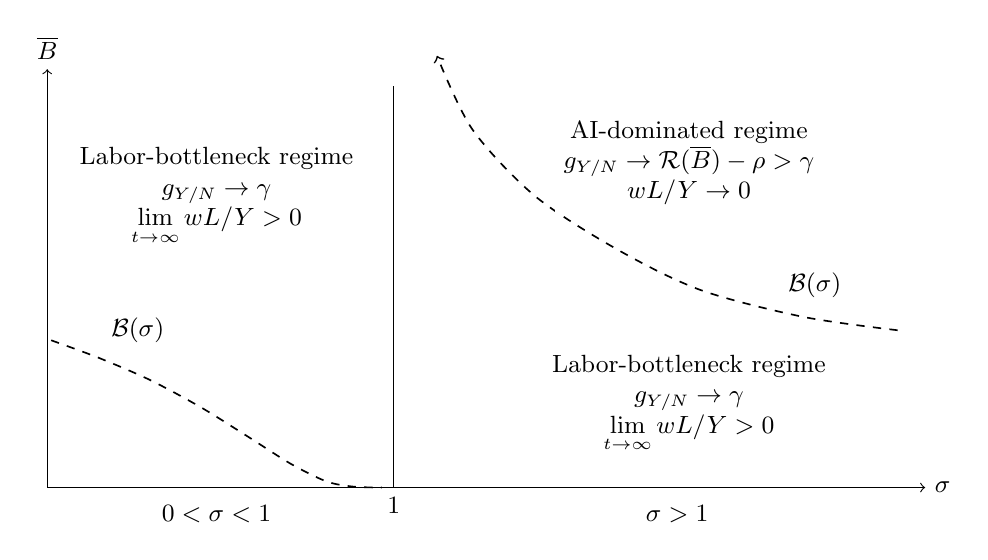
\begin{tikzpicture}[
 x=1.00cm,y=0.85cm,
 every node/.style={font=\small},
 regime/.style={align=center,inner sep=3pt,fill=white}
]
 \draw[->] (0,0) -- (11.15,0) node[right] {$\sigma$};
 \draw[->] (0,0) -- (0,6.25) node[above] {$\overline B$};
 \draw[semithick] (4.40,0) -- (4.40,6.00);
 \node[below] at (4.40,0) {$1$};
 \node[below] at (2.15,-0.12) {$0<\sigma<1$};
 \node[below] at (8.00,-0.12) {$\sigma>1$};

 % The complementary branch approaches zero as sigma approaches one
 % from below. It is not a continuation of the gross-substitutes branch.
 \draw[semithick,dashed]
  plot[smooth] coordinates
  {(0.05,2.20) (0.65,1.94) (1.30,1.61) (1.95,1.20)
   (2.55,0.76) (3.10,0.35) (3.55,0.09) (3.90,0.012)
   (4.25,0.001)};
 \node[regime] at (2.15,4.35)
  {Labor-bottleneck regime\\
   $g_{Y/N}\to\gamma$\\
   $\displaystyle\lim_{t\to\infty}wL/Y>0$};
 \node[regime] at (1.15,2.35) {$\mathcal B(\sigma)$};

 \draw[semithick,dashed,->]
  plot[smooth] coordinates
  {(10.80,2.35) (9.60,2.55) (8.30,2.95) (7.25,3.55)
   (6.20,4.35) (5.40,5.35) (4.95,6.45)};

 \node[regime] at (8.15,4.85)
  {AI-dominated regime\\
   $g_{Y/N}\to \mathcal R(\overline B)-\rho>\gamma$\\
   $wL/Y\to0$};
 \node[regime] at (8.15,1.25)
  {Labor-bottleneck regime\\
   $g_{Y/N}\to\gamma$\\
   $\displaystyle\lim_{t\to\infty}wL/Y>0$};
 \node[regime] at (9.75,3.02) {$\mathcal B(\sigma)$};
\end{tikzpicture}%
}
\caption{Growth regimes with an upper bound on AI efficiency. %For $0<\sigma<1$, $\overline B>\mathcal B(\sigma)$ is the condition for the positive-labor-share construction in Proposition~\ref{prop:rewrite-capped-complements-existence}. For $\sigma>1$, the curve separates the labor-bottleneck and AI-dominated equilibria in Proposition~\ref{prop:rewrite-capped-substitutes-labor-existence} and~\ref{prop:rewrite-capped-substitutes-existence}.
}
\label{fig:rewrite-frontier-regimes}
\end{figure}


Table~\ref{tab:rewrite-finite-existence} summarizes the four cases of Proposition~\ref{prop:rewrite-equilibrium-regimes}. For $\sigma>1$, an upper bound below $\mathcal B(\sigma)$ makes the return on capital at a vanishing labor share too low for capital and AI services to outgrow effective labor. Above the threshold, that return supports their faster growth along the AI-dominated equilibria. Across these equilibrium regimes, long-run wage growth exceeds $\gamma$ if and only if labor's income share converges to zero. %Proposition~\ref{prop:rewrite-output-wage-wedge} in Appendix~\ref{app:rewrite-proofs} derives the exact relationship between the wage-growth premium and the decline in labor's income share.


\begin{table}[H]
\centering
\caption{Long-run equilibrium characterization}
\label{tab:rewrite-finite-existence}
\small
\begin{tabular}{@{}cccccc@{}}
\toprule
Elasticity & AI efficiency bound & $\lim g_{Y/N}$ & $\lim g_w$ & $\lim wL/Y$ & $\lim r$ \\
\midrule
$0<\sigma<1$ & $\overline B>\mathcal B(\sigma)$ & $\gamma$ & $\gamma$ & Positive & $\rho+\gamma$ \\
$\sigma=1$ & Any finite $\overline B$ & $\gamma$ & $\gamma$ & $(1-\alpha)\omega_L$ & $\rho+\gamma$ \\
$\sigma>1$ & $\overline B<\mathcal B(\sigma)$ & $\gamma$ & $\gamma$ & Positive & $\rho+\gamma$ \\
$\sigma>1$ & $\overline B>\mathcal B(\sigma)$ & $\mathcal R(\overline B) -\rho$ & $\gamma+\frac{\mathcal R(\overline B)-\rho-\gamma}{\sigma}$ & Zero & $\mathcal R(\overline B)$ \\
\bottomrule
\end{tabular}
\end{table}


%I use this comparison as an economic regime threshold only for $\sigma>1$. For $\sigma<1$, $s_X\to1$ corresponds instead to AI services becoming scarce relative to effective labor. The condition $\overline B>\mathcal B(\sigma)$, or $\mathcal R(\overline B)>\rho+\gamma$, is then only a sufficient condition for the positive-labor-share construction in Proposition~\ref{prop:rewrite-capped-complements-existence}; it does not imply AI-dominated growth.


%Section~\ref{sec:rewrite-uncapped} studies the economy without an upper bound on AI efficiency. Those results require a separate equilibrium analysis.
